\documentclass{beamer}

\newcommand{\course}{CS 1331 Introduction to Object Oriented Programming}
\newcommand{\lesson}{{\tt Java Collections (Part 2 of 3)}}
\newcommand{\code}{http://www.cc.gatech.edu/~simpkins/teaching/gatech/cs1331/code}

\author[Chris Simpkins]
{Christopher Simpkins \\\texttt{chris.simpkins@gatech.edu}}
\institute[Georgia Tech] % (optional, but mostly needed)

\date[CS 1331]{}


\newcommand{\course}{Introduction to Object-Oriented Programming}
\subject{\course}
\title[\lesson]{\course}
\subtitle{\lesson}

\author[CS 1331]
{Christopher Simpkins \\\texttt{chris.simpkins@gatech.edu}}
\institute[Georgia Tech]

\date[]{}

\newcommand{\link}[2]{\href{#1}{\textcolor{blue}{\underline{#2}}}}
\newcommand{\code}{http://www.cs1331.org/code}

\usepackage{colortbl}

% If you have a file called "university-logo-filename.xxx", where xxx
% is a graphic format that can be processed by latex or pdflatex,
% resp., then you can add a logo as follows:

% \pgfdeclareimage[width=0.6in]{coc-logo}{cc_2012_logo}
% \logo{\pgfuseimage{coc-logo}}

\mode<presentation>
{
  \usetheme{Berlin}
  \useoutertheme{infolines}

  % or ...

 \setbeamercovered{transparent}
  % or whatever (possibly just delete it)
}

\usepackage{tikz}
% Optional PGF libraries
\usepackage{pgflibraryarrows}
\usepackage{pgflibrarysnakes}
\usepackage{pgfplots}
\usepackage{fancybox}
\usepackage{listings}
\usepackage{hyperref}
\hypersetup{colorlinks=true,urlcolor=blue}
\usepackage[english]{babel}
% or whatever

\usepackage[latin1]{inputenc}
% or whatever

\usepackage{times}
\usepackage[T1]{fontenc}
% Or whatever. Note that the encoding and the font should match. If T1
% does not look nice, try deleting the line with the fontenc.


\usepackage{listings}

% "define" Scala
\lstdefinelanguage{scala}{
  morekeywords={abstract,case,catch,class,def,%
    do,else,extends,false,final,finally,%
    for,if,implicit,import,match,mixin,%
    new,null,object,override,package,%
    private,protected,requires,return,sealed,%
    super,this,throw,trait,true,try,%
    type,val,var,while,with,yield},
  otherkeywords={=>,<-,<\%,<:,>:,\#,@},
  sensitive=true,
  morecomment=[l]{//},
  morecomment=[n]{/*}{*/},
  morestring=[b]",
  morestring=[b]',
  morestring=[b]""",
}

\usepackage{color}
\definecolor{dkgreen}{rgb}{0,0.6,0}
\definecolor{gray}{rgb}{0.5,0.5,0.5}
\definecolor{mauve}{rgb}{0.58,0,0.82}

% Default settings for code listings
\lstset{frame=tb,
  language=scala,
  aboveskip=2mm,
  belowskip=2mm,
  showstringspaces=false,
  columns=flexible,
  basicstyle={\scriptsize\ttfamily},
  numbers=none,
  numberstyle=\tiny\color{gray},
  keywordstyle=\color{blue},
  commentstyle=\color{dkgreen},
  stringstyle=\color{mauve},
  frame=single,
  breaklines=true,
  breakatwhitespace=true,
  keepspaces=true
  %tabsize=3
}


% If you wish to uncover everything in a step-wise fashion, uncomment
% the following command:

% \beamerdefaultoverlayspecification{<+->}


\begin{document}

\begin{frame}
  \titlepage
\end{frame}


%------------------------------------------------------------------------
\begin{frame}[fragile]{The Collections Framework}

\begin{center}
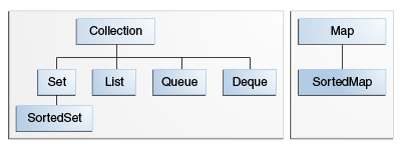
\includegraphics[width=4in]{colls-coreInterfaces.png}
\end{center}

\begin{itemize}
\item A {\it collection} is an object that represents a group of objects.
\item The collections framework allows different kinds of collections to be dealt with in an implementation-independent manner.
\end{itemize}


\end{frame}
%------------------------------------------------------------------------

%------------------------------------------------------------------------
\begin{frame}[fragile]{{\tt Collections.sort(List<T> list)}}


The collections framework includes algorithms that operate on collections.  These algorithms are implemented as static methods of the {\tt Collections} class.  A good example is the (overloaded) {\tt sort} method:
\begin{lstlisting}[language=Java]
public static <T extends Comparable<? super T>> void sort(List<T> list)
\end{lstlisting}
This method signature demonstrates how to declare a generic method (so far we've seen only generic classs): put a type parameter before the return type.
\begin{itemize}
\item This {\tt sort} uses the ``natural ordering'' of the list, that is, the ordering defined by {\tt Comparable}.
\item {\tt <? super T>} is a {\it type bound}.  It means ``some superclass of {\tt T}.''
\item The type parameter {\tt <T extends Comparable<? super T>>} means that the element type {\tt T} or some superclass of {\tt T} must implement {\tt Comparable}.
\end{itemize}


\end{frame}
%------------------------------------------------------------------------

%------------------------------------------------------------------------
\begin{frame}[fragile]{The {\tt java.lang.Comparable} Interface}


\begin{lstlisting}[language=Java]
public interface Comparable<T> {

    public int compareTo(T o);
}
\end{lstlisting}

{\tt compareTo(T o)} Compares this object with the specified object for order. Returns
\begin{itemize}
\item a negative integer if this object is less than the other object,
\item zero if this object is equal to the other object, or
\item a positive integer if this object is greater than the other object.
\end{itemize}

\end{frame}
%------------------------------------------------------------------------

%------------------------------------------------------------------------
\begin{frame}[fragile]{Implementing {\tt java.lang.Comparable<T>}}


Here's a {\tt Person} class whose natural ordering is based on age:
\begin{lstlisting}[language=Java]
public class Person implements Comparable<Person> {

    private String name;
    private int age;

    public Person(String name, int age) {
        this.name = name;
        this.age = age;
    }

    public String toString() {
        return name;
    }

    public int compareTo(Person other) {
        return this.age - other.age;
    }
}
\end{lstlisting}


\end{frame}
%------------------------------------------------------------------------

%------------------------------------------------------------------------
\begin{frame}[fragile]{Using {\tt Collections.sort(List<T> list)}}


Given the {\tt Collections} static method:
\begin{lstlisting}[language=Java]
public static <T extends Comparable<? super T>> void sort(List<T> list)
\end{lstlisting}

We could sort a {\tt List<Person>} because {\tt Person implements Comparable<Person>}:
\begin{lstlisting}[language=Java]
List<Person> peeps = new ArrayList<>();
peeps.add(new Person(...));
...
Collections.sort(peeps);
\end{lstlisting}
And if we have a class:
\begin{lstlisting}[language=Java]
public class GtStudent extends Person { ... }
\end{lstlisting}

We could also sort a {\tt List<GtStudent>} becuase
\begin{itemize}
\item {\tt GtStudent extends Person},
\item {\tt Person implements Comparable<Person>} and
\item {\tt Person} is a supertype of {\tt GtStudent}
\end{itemize}

\end{frame}
%------------------------------------------------------------------------

%------------------------------------------------------------------------
\begin{frame}[fragile]{Using {\tt Collections.sort(List<T>)} on Raw Lists}

Java uses {\it type erasure} to implement generics, meaning that the compiled code is nearly identical to non-generic code.  Type erasure allows for compile-time type checking while preserving the ability to work with legacy code.  So you can sort a raw {\tt List} of {\tt Person} using the {\tt compareTo(Person)} method:

\begin{lstlisting}[language=Java]
List rawPeeps = new ArrayList();
rawPeeps.add(new Person(...));
...
Collections.sort(rawPeeps);
\end{lstlisting}

Overriding only happens when methods have identical signatures.  To allow generic classes to work in non-generic settings, the compiler inserts {\it bridge} methods.  So {\tt Person} looks like:

\begin{lstlisting}[language=Java]
public class Person implements Comparable<Person> {
    // ...

    // This is a bridge method inserted by the compiler to allow this
    // class to work with legacy non-generic code
    public int compareTo(Object other) {
        return compareTo((Person) other);
    }

    public int compareTo(Person other) {
        return this.age - other.age;
    }
}
\end{lstlisting}

\end{frame}
%------------------------------------------------------------------------

%------------------------------------------------------------------------
\begin{frame}[fragile]{Using {\tt Collections.sort(List<T>)} on Raw Lists}

Overriding only happens when methods have identical signatures.  To allow generic classes to work in non-generic settings, the compiler inserts {\it bridge} methods.  So {\tt Person} looks like:

\begin{lstlisting}[language=Java]
public class Person implements Comparable<Person> {
    // ...

    // This is a bridge method inserted by the compiler to allow this
    // class to work with legacy non-generic code
    public int compareTo(Object other) {
        return compareTo((Person) other);
    }

    public int compareTo(Person other) {
        return this.age - other.age;
    }
}
\end{lstlisting}

\end{frame}
%------------------------------------------------------------------------


%------------------------------------------------------------------------
\begin{frame}[fragile]{Using {\tt java.util.Comparator<T>}}


\begin{lstlisting}[language=Java]
public interface Comparator<T> {

    int compare(T o1, T o2);

    boolean equals(Object obj);
}

\end{lstlisting}

{\tt Comparator<T>} is an interface with two methods:
\begin{itemize}
\item {\tt int compare(T o1, T o2)} -  same contract as {\tt o1.compareTo(o2)}
\item {\tt boolean equals(Object obj)}
\end{itemize}
It's always safe to use the inherited {\tt equals} method, so the one you need to implement is {\tt compare}.\\

See \link{\code/SuperTroopers.java}{SuperTroopers.java} for examples using {\tt Comparable}, {\tt Comparator} and {\tt Collections.sort(...)}.

\end{frame}
%------------------------------------------------------------------------


%------------------------------------------------------------------------
\begin{frame}[fragile]{Programming Exercise}

Write a class to represent Georgia Tech students called, say, {\tt GtStudent}.
\begin{itemize}
\item Give {\tt GtStudent} name, major, GPA, and year fields/properties.
\item Have {\tt GtStudent} implement {\tt Comparable<T>} with some ordering that makes sense to you -- perhaps some majors are harder than others, so GPAs are adjusted in comparisons.
\item Add instances of {\tt GtStudents} to an {\tt ArrayList<E>}.
\item Sort the {\tt ArrayList} of {\tt GtStudent}s using {\tt Collections.sort(List<E>)}.
\item Write a {\tt Comparator<GtStudent>} and sort your list with {\tt Collections.sort(List<E>, Comparator<E>)}.
\end{itemize}
Extra: add thousands of randomly-gnerated {\tt GtStudent}s to an {\tt ArrayList} and a {\tt LinkedList} and time {\tt Collections.sort(List<E>)} method invocations for each of them.  Is one faster?  Why (or why not)?

\end{frame}
%------------------------------------------------------------------------


% %------------------------------------------------------------------------
% \begin{frame}[fragile]{}


% \begin{lstlisting}[language=Java]

% \end{lstlisting}

% \begin{itemize}
% \item
% \end{itemize}


% \end{frame}
% %------------------------------------------------------------------------


\end{document}
